\chapter{Wireless Channel Modeling}
\label{chap:ChannelModeling}
% TODO: Introduce Fadnig impairments following
% Simulation of Communication Systems

% TODO: give the text book description of large scale fading
\newpage
\section{Fading Channels}

Fading is a major component of wireless channel %
impairments. Fading comes under two main categories %
large scale and small scale fading. Figure \ref{fig:Fading} %
illustrates these two main components of fading.
\FloatBarrier
\begin{figure}[h!]
	\centering
	\includegraphics[width=\textwidth,
		height=\textheight, keepaspectratio]
		{./Figures/%
		WirelessChannel/LargeandSmallScale%	
		Fading.png}
	\caption{combination of large and small %
		scale fading (a) and the small-scale %
		fading component (b) from %
		\cite{Sklar97-1}}
	\label{fig:Fading}
\end{figure}

\FloatBarrier
\subsection{Large Scale Fading}

Large scale fading, also sometimes referred to as %
shadow fading is characterised by an attenuation %
of the average signal power as can be seen in %
figure \ref{fig:Fading}a). It is caused %
by significant obstructions to the signal such as %
buildings or hills between the transmitter and %
receiver. The receiver is therefore being %
\emph{shadowed} by the obstruction. 

The received signal power can be modeled as:

\begin{align}
	S_{r} = S_{t} + G_{t} + G_{r} - L_{p}
\end{align}

Where $S_{r}$ is the received signal power in dB, %
$S_{t}$ is the transmit signal power in dB, $G_{t}$ 
and $G_{r}$ are the transmit and receive antenna %
gains in dB and $L_{p}$ is the propagation loss in dB. %
Typically $S_{r}$, $S_{t}$, $G_{t}$, and $G_{r}$ are %
either well known or are easily modeled, in the case of %
fading channels the propagation loss is the most difficult %
to predict \cite{Jer00}. There are two main methods %
of attempting to model $L_{p}$, ray tracing methods %
which must be location specific and statistical models. %
I will constrain this section to the development of %
statistical models. 

The most popular of the statistical models are the %
class of slope-intercept models \cite{Jer00}. These %
models treat propagation loss as being composed of %
a deterministic component and a statistical component.

\begin{align}
	L_{p} = \alpha + \beta log_{10}(R) + \gamma \text{ dB}
\end{align}

where $R$ is the distance from the transmitter to the %
receiver in kilometres, $\alpha$ and $\beta$ are parameters %
determined by the model, and $\gamma$ is the %
statistical component of the model. Values for $\alpha$ and %
$\beta$ are determined from experimental measurements %
where received signal power averaged over several %
wavelengths are taken over many different locations %
around the transmitter. These received signal %
powers can be plotted against the log of %
the distance to the transmitter and a least squares fit %
can be made to the data. The resulting residuals around %
the least squares fit describes $\gamma$.

Some well-known slope intercept models are the Hata%
\cite{Hata80} model and the COST-231 model\cite{COST231}.

Typically the residuals  of the slope intercept models %
when measured in dB follow a gaussian distribution with %
zero mean and a standard deviation of about 8dB\cite{Jer00}.
So the large scale fading follows a log-normal distribution.

\subsection{Small Scale Fading}

Small scale fading, also commonly referred to as multipath %
fading is caused by the transmitted signal following many %
different paths before arriving at the receiving antenna. %
Each of these multiple paths can have different lengths %
and may be reflected or refracted many times, a process %
typically referred to as scattering. As a result of the %
varying distances each propagation path takes, the time %
taken for a transmitted waveform to reach the receiver %
is also going to vary down each of these paths, figure %
\ref{fig:MultipathChannel} illustrates this multipath %
behaviour.

\begin{figure}[ht]
	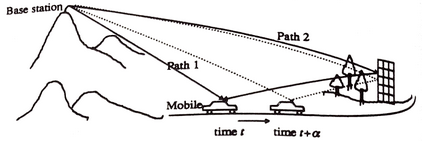
\includegraphics[width=\textwidth]{./Figures/%
		WirelessChannel/MultipathChannel.png}
	\caption{Multipath Channel \cite{Jer00}}
	\label{fig:MultipathChannel}
\end{figure} 

The resulting effect of this multipath channel is that %
symbols transmitted at different times will arrive %
at the receiver at the same time, this leads to %
a self-interfering effect that can cause the received %
signal power to undergo large fluctuations and can %
be characterised as inter-symbol interference.

The multipath fading can be broadly organised into %
two separate categories\cite{Jer00}.

\begin{enumerate}
	\item{The multipath signal paths are made up %
		of relatively small and identifiable number %
		of components reflected by small hills, %
		houses, and other strucutres encountered in %
		open areas and rural environments. This %
		results in a channel model with a finite number %
		of multipath components. Such a channel is %
		referred to as a \emph{discrete multipath channel}.}
	\item{The multipath signal paths are generated by %
		a large unresolvable reflections as might occur %
		in a mountainous area or in a dense urban environment. %
		This signal is composed of a continuum of %
		unresolvable multipath components. This %
		channel model is referred to as a \emph{diffuse %
		multipath channel}.}
\end{enumerate}

Multipath reflected components can be described in %
terms of orthogonal components $x_{n}(t)$ and %
$y_{n}$%
(t), where $x_{n}(t) + jy_{n}(t) = \alpha_{n}(t)e^{%
-j\theta_{n}(t)}$. If the number of random components %
is large enough and none are dominant, then the received %
components $x_{r}(t)$ and $y_{r}(t)$ which are the sums %
of the reflected signals will have a gaussian probability %
density function. The magnitude of the received scattered %
components will have a magnitude described by:

\begin{align}
	r_{0}(t) = \sqrt{x_{r}^{2}(t) + y_{r}^{2}(t)}
\end{align}

The probability density function of the envelope $r_{0}(t)$ %
of the received signal is going to follow a Rayleigh distribution %
with probability density function:

\begin{align}
	f_{R}(r_{0}) = \begin{cases}
		\frac{r_{0}}{\sigma^{2}}e^{-r_{0}^{2}/(2\sigma^{2})} %
		& \text{ for } r_{0} \geq 0 \\
		0 & \text{ otherwise}
	\end{cases}
	\label{eq:RayleighPDF}
\end{align}

Where $\sigma^{2}$ is the mean power of the received %
multipath signal. This type of fading is called Rayleigh %
fading.

\begin{figure}[h!]
	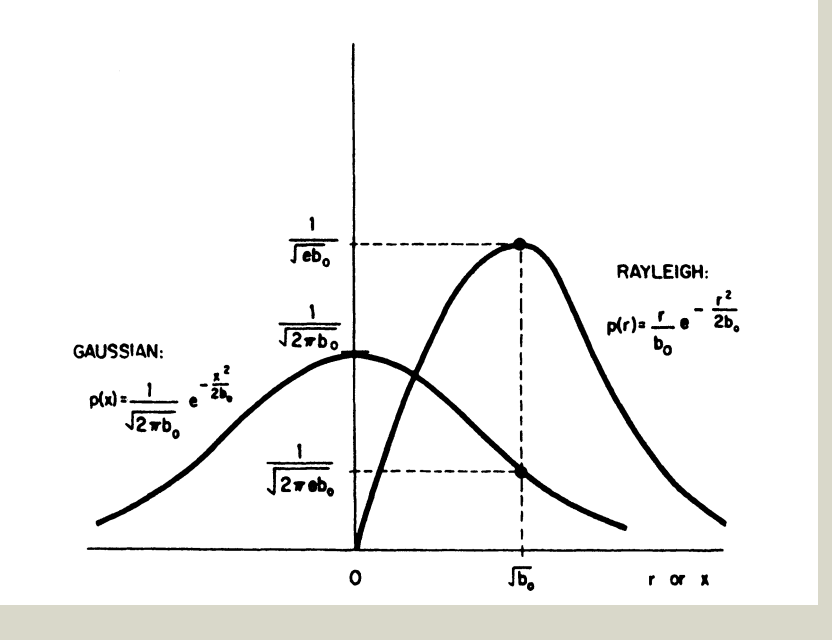
\includegraphics[width=\linewidth]{./Figures/%
	WirelessChannel/RayleighDistribution.png}
	\caption{Gaussian and Rayleigh Distributions%
	\cite{Jakes74}}
	\label{fig:RayleighDistribution}
\end{figure}

Figure \ref{fig:RayleighDistribution} illustrates %
the gaussian distribution and the rayleigh %
distribution.

When the received signal is made up of multiple %
reflected rays and a significant line-of-sight %
component, the received envelope ampliude %
follows a Rician distribution with probability density %
function:

\begin{align}
	f_{R}(r_{0}) = \begin{cases}
		\frac{r_{0}}{\sigma^{2}}I_{0}%
		\left[ \frac{A_{r}}{\sigma^{2}} \right]%
		e^{-(r_{0}^{2}-A^{2})/(2 \sigma^{2})}%
		 & \text{ for } r_{0} \geq 0, A \geq 0\\
		0 & \text{ Otherwise}
	\end{cases}
	\label{eq:RicianPDF}
\end{align}

where $I_{0}$ is the modified zeroth order %
bessel function of the first kind. This kind of %
fading is commonly referred to as Rician fading. %
The Rician distribution is commonly described in %
terms of a parameter K\cite{Sklar01}, which is defined as %
the ratio of power in the specular component to the %
power in the multipath signal and is given as:

\begin{align}
	K = \frac{A^{2}}{2\sigma^{2}}
\end{align}

Figure \ref{fig:RicianDistribution} illustrates the relationship %
of the rician probability density function to the rayleigh %
PDF with respect to mean specular signal amplitude $v$ and %
mean scattered signal power of $1$.

\begin{figure}[ht]
	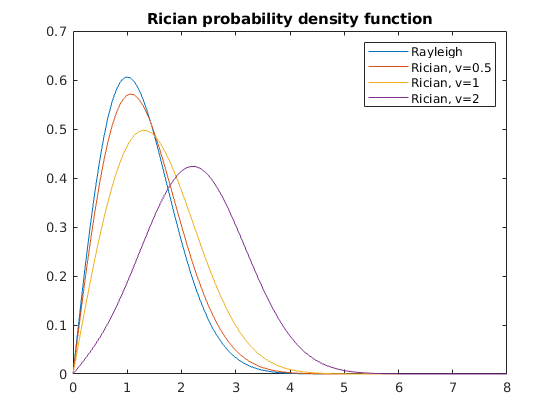
\includegraphics[width=\linewidth]{./Figures/%
	WirelessChannel/RicianDistribution.png}
	\caption{Rayleigh and Rician Probability %
	Density Function}
	\label{fig:RicianDistribution}
\end{figure}

\section{Time and Frequency Characteristics of Fading %
Channels}
\FloatBarrier

Figure \ref{fig:FadingBlocks} provides a broad %
description of the important components within %
fading channels. In this section we will draw our %
attention to blocks $5$ and $6$ under small %
scale fading.

\begin{figure}[ht]
	\includegraphics[width=\textwidth]{./Figures/%
		WirelessChannel/FadingBlockDiagram%
		.png}
	\caption{Fading Channel manifestations%
		\cite{Sklar97-1}}
	\label{fig:FadingBlocks}
\end{figure}

As is apparent from the diagram, small-scale fading %
can be described by two key components, the time %
spreading of the signal or dispersion, and the time %
variance of the channel. 

Bello \cite{Bello63} proposed a simple wide-sense %
stationary uncorrelated scattering model of fading in %
1963. This model treats the received signals arriving %
with different delays as being uncorrelated and that %
the channel is wide sense stationary in both the time %
and frequency domains. Using this model four functions %
can be defined that characterise the fading as shown in %
figure \ref{fig:FadingFunctions}.

\begin{figure}[ht]
	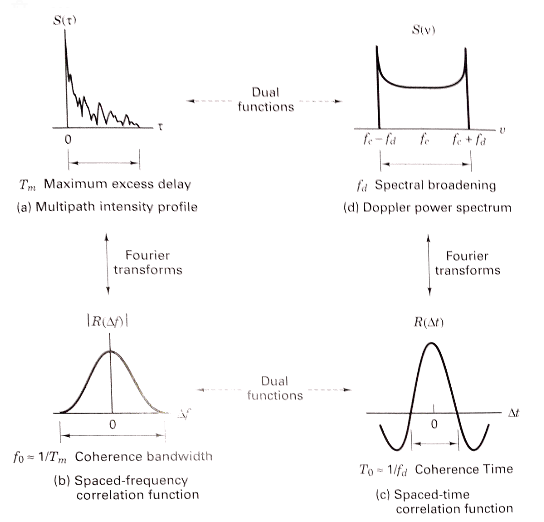
\includegraphics[width=\textwidth]{./Figures/%
		WirelessChannel/FadingFunctions.png}
	\caption{Four Functions that define Fading in %
			a WSSUS channel \cite{Sklar01}}
	\label{fig:FadingFunctions}
\end{figure}

\FloatBarrier
\subsection{Time Spreading}
In this section we will focus on figure %
\ref{fig:FadingFunctions}a) and \ref{%
fig:FadingFunctions}b). The multipath %
intensity profile also referred to as the %
power delay profile plots the received %
signal power vs the excess delay. %
Excess delay is defined as the propagation %
delay of the signal that exceeds the delay %
of the first signal arrival at the receiver %
\cite{Sklar01}.

In the fading channel, the maximum excess %
excess delay time $T_{m}$ and symbol time %
$T_{m}$ can be used to categorise the %
fading into two categories:

\begin{itemize}
	\item{frequency-selective fading}
	\item{frequency nonselective or flat fading}
\end{itemize}

The channel is frequency selective when %
$T_{m} > T_{s}$. This occurs when the %
excess delay induced by the multipath %
components of the symbol last longer %
than the symbols time duration. This leads %
to an effect where the multipath components %
of one symbol can interfere with the next symbol. %
This effect is named channel induced ISI. The %
channel exhibits flat fading when %
$T_{m} < T_{s}$. This is when %
the multipath components of a symbol %
all arrive within the symbol time, the multipath %
components are all contained within the symbol and %
do not interfere with neighbouring symbols so ISI %
does not happen, there is however still signal %
degradation since the multipath components still %
self-interfere.

This same time spreading effect can be analysed in %
the frequency domain. If the fourier transform of %
$S(\tau)$ illustrated in figure \ref{fig:FadingFunctions}a) %
is taken then the function $\lvert %
R(\Delta f) \rvert$ as illustrated in figure %
\ref{fig:FadingFunctions}b) is revealed. This function, %
referred to as the \emph{spaced-frequency correlation %
function} represents the correlation between the channel %
response to two signals as a function of frequency %
difference between the two signals. It can be thought of %
as the frequency transfer function of the channel and so %
the time spreading effect can be understood as the result %
of the channel filter.
\FloatBarrier
The spaced-frequency correlation function allows us to %
understand the similarity between two received signal %
that are spaced in frequency $\Delta f = f_{1} - f_{2}$. %
Frequency selective fading can be understood as the %
spaced-frequency correlation function is poorly correlated %
across the signal bandwidth, and flat fading can be understood %
as the spaced-frequency correlation function being highly %
correlated across the signal bandwidth. An important %
parameter, the \emph{coherence bandwidth} $f_{0}$ %
can be used as a statistical measure of the bandwidth %
of which the signal of interest experiences equal gain %
and linear phase. $f_{0}$ and $T_{m}$ are reciprocally %
related and as an approximation

\begin{align}
	f_{0} \approx \frac{1}{T_{m}}
\end{align}

\begin{figure}[ht]
	\includegraphics[width=\textwidth]{./Figures/%
		WirelessChannel/FrequencyCoherence%
		.png}
	\caption{frequency selective and flat fading %
	\cite{Sklar01}}
	\label{fig:FadingFigure}
\end{figure}

Figure \ref{fig:FadingFigure} illustrates the difference %
between frequency selective and flat fading in the %
frequency domain. $W$ is the transmitted signal %
bandwidth and $f_{0}$ is the coherence bandwidth.
\FloatBarrier
The maximum excess delay $T_{m}$ is not always the %
best indicator of channel performance, as channels with %
different $T_{m}$ can exhibit different power delay profiles. %
A different parameter that is used for understanding %
coherence bandwidth is the root-mean-squared delay spread.

\begin{align}
	\sigma_{\tau} = \sqrt{\overline{\tau^{2}} - (\bar{\tau}^{2})}
\end{align}

where $\overline{\tau^{2}}$ and $\bar{\tau}^{2}$ are defined %
as:

\begin{align}
	\overline{\tau^{2}} =&  \frac{\int \tau^{2} S(\tau) d\tau}{\int S(\tau) d\tau} \\
	\bar{\tau} =& \frac{\int \tau S(\tau) d\tau}{\int S(\tau) d\tau}
\end{align}

Using this rms delay a popular approximation of %
the coherence bandwidth where the correlation %
of the signal within this bandwidth is at least 0.5 is

\begin{align}
	f_{0} \approx \frac{1}{5\sigma_{\tau}}
\end{align}

\subsection{Time Variance}
Time variance of the channel is caused by relative %
motion between the transmitter and receiver or by %
objects moving about within the channel \cite{Sklar01}. %
Figure \ref{fig:FadingFunctions}c) shows the function %
$R(\Delta t)$ named the \emph{spaced-time correlation %
function}. Similar to the spaced-frequency correlation %
function $R(\Delta t)$ measures the similarity between %
two signals in the \emph{time} domain. It's measured %
by sending two sinusoids through the channel at differing %
times $\Delta t = t_{1} - t_{2}$ and evaluating their %
cross correlation. 

Just as the spaced-frequency correlation function has a %
measure of coherence bandwidth, the spaced-time %
correlation function has a measure of \emph{coherence %
time} $T_{0}$. The coherence time is a measurement of %
the duration the channel is invariant. 

The coherence time of the channel allows the fading %
to be categorised two ways as in figure \ref{fig:FadingBlocks}, %
blocks 14, 15, 17, 18.

\begin{itemize}
	\item{fast fading}
	\item{slow fading}
\end{itemize}

Fast fading occurs when the coherence time $T_{0}$ %
is less than the symbol time $T_{s}$ ie.

\begin{align}
	T_{0} < T_{s}
\end{align}

Slow fading occurs whne the coherence time is %
greater than the symbol time

\begin{align}
	T_{0} > T_{s}
\end{align}

In fast fading the received signal pulse undergoes %
distortion that leaves it uncorrelated throughout time. %
A slow fading channel does not induce this pulse distortion %
as the channel is relatively invariant throughout one symbol %
period.

It's been shown \cite{Clarke68} that under the popular %
dense scatterer model the normalized $R(\Delta t)$ is

\begin{align}
	R(\Delta t) = J_{0}(kV \Delta t)
\end{align}

where $J_{0}(\cdot)$ is the zeroth order Bessel %
function of the first kind. $V$ is the relative velocity %
between the transmitter and receiver and %
$k = \frac{2\pi}{\lambda}$ is the free-space %
phase constant. An interesting point about %
this expression is that it can be expressed both %
in time or distance (where distance is $V\Delta t$). %
It has been shown \cite{Amoroso96} that at a %
distance of $0.38\lambda$ from the point of %
reference that the combined magnitudes and %
phases of a continuous wave signal are %
statistically uncorrelated.

The frequency domain interpretation of %
this time variation is that of a doppler-shift %
represented in the frequency domain. Figure %
\ref{fig:FadingBlocks}d) shows the \emph{%
Doppler power spectral density} or simply %
Doppler spectrum. For the case of the dense %
scatterer model, a vertical receive antenna with %
constant azimuthal gain, a uniform distribution of %
signals arriving at all arrival angles, and an a %
continuous wave signal the doppler spectrum is %
\cite{Clarke68}

\begin{align}
	S(\nu) = \frac{1}{\pi f_{d} \sqrt{1 - %
		(\frac{\nu - f_{c}}{f_{d}})^{2}}}
\end{align}

Where $\nu$ is the frequency shift, $f_{d}$ is the %
doppler frequency and $f_{c}$ is the carrier frequency. %
This spectrum is known as the Jakes' spectrum\cite{Iskander}. %
The doppler shift is the result of the fourier transform %
of the spaced-time correlation function similar to how %
the spaced-frequency correlation function is the %
Fourier transform of the power delay profile. The %
shape of this spectrum is bowl shaped as can be seen in %
figure \ref{fig:FadingFunctions}d).

The magnitude of the doppler shift is given by:

\begin{align}
	f_{d} = \frac{V}{\lambda}
\end{align}

where $V$ is the relative velocity between the %
transmitter and receiver and $\lambda$ is the signal %
wavelength.

\section{Wireless Channel as a Filter}

Multipath fading can be modeled as a kind of %
finite impulse response filter where each %
sample at the receiver is a linear combination %
of the samples transmitted over the multipath %
channel.

\begin{align}
	y(t) = \sum_{n} \alpha_{n}(t)s(t-\tau_{n}(t))
	\label{eq:ChannelFIR}
\end{align}

where $s(t)$ is the bandpass input signal, $\alpha_n(t)$ %
is the attenuation factor for the signal received %
on the $n\text{th}$ path, and $\tau_n(t)$ is the %
propagation delay along that path. A natural model %
for equation \ref{eq:ChannelFIR} is that of a %
tapped-delay line with time-varying coefficients. %
If the bandpass signal $s(t)$ is represented as:

\begin{align}
	s(t) = Re\left\{ \tilde{s}%
	(t)e^{j2\pi f_{c} t} \right\}
\end{align}

where $\tilde{s}$ is the complex baseband signal. %
Then the channel output $y(t)$ can be represented as:

\begin{align}
	y(t) = Re\left\{\left( \sum_{n} %
	\alpha_{n}(t) e^{-j2 \pi f_{c} \tau_{n}(t)} %
	\tilde{s}(t - \tau_{n}(t)) \right)%
	e^{j 2\pi f_{c} t} \right\}
\end{align}

the complex envelope of $y(t)$ is:

\begin{align}
	\tilde{y}(t) =& \sum_{n}\alpha_{n}(t)%
	e^{-j 2\pi f_{c} \tau_{n}(t)} %
	\tilde{s}(t - \tau_{n}(t))
		     =& \sum_{n}%
	\tilde{\alpha}_{n}(t)\tilde{s}(%
	t-\tau_{n}(t))
	\label{eq:ChannelOutput}
\end{align}

Equation \ref{eq:ChannelOutput} makes it clear that %
the channel response can be represented using a %
complex, baseband equivalent impulse response.

\begin{align}
	\tilde{h}(\tau;t) = \sum_{n} %
	\alpha_{n}(t)\delta(\tau - %
	\tau_{n}(t))
\end{align}

where the output is
% I need to check this with the latest textbook
% When I get home.
\begin{align}
	\tilde{y}(t) = \sum_{n} \tilde{h}%
	(\tau;t)\tilde{s}(t - \tau)
	\label{eq:BasebandChannelFIR}
\end{align}

If $h(\tau;t)$ was time-invariant this would be the %
equivalent of a normal convolution sum.


% TODO: Develop the mathematics of the finite gaussian channel model


